\section{Introduction}
%%%%%%%%%%%%%%%%%%%%%%%%%%%%%%%%%%%%%%%%%%%%%%%%%%%%%%%%%%%%%%%%%%%%%%
\label{sec:Introduction}

%This measurement can be used to directly inspect the perturbative QCD theory in the Higgs sector.
%In particular the \pth variable is sensitive to the Higgs production mode and the differential distribution in this variable can be used to inspect the effects of the top quark mass in the gluon fusion top loop. Moreover, any observed deviation from the SM expectation, especially in the tail of the \pth distribution, could be a hint of physics beyond the SM.

\begin{comment}
The Higgs boson production at hadron colliders is characterized by the Higgs boson transverse momentum, \pth, and its pseudorapidity, $\eta$. The $\eta$ distribution is essentially driven by the PDF of the partons in the colliding hadrons, and it is only mildly sensitive to radiative corrections. The \pth distribution is instead sensitive to QCD radiative corrections. 
Considering the ggH production mode, at LO in perturbation theory, $\mathcal{O}(\alpha_s^2)$, the Higgs boson is always produced with \pth equal to zero. Indeed in order to have \pt different from zero, the Higgs boson has to recoil at least against one parton. Higher order corrections to the ggH process are numerically large and are known at NLO including full top quark mass dependence~\cite{Spira:1995rr,Harlander:2005rq}, and at NNLO using the so-called large-$m_\mathrm{t}$ approximation~\cite{Ravindran:2003um,Catani:2007vq,Anastasiou:2015ema}, in which the top quark mass is assumed to be very large and the fermionic loop is replaced by an effective vertex of interaction. Starting from the NLO, the Higgs boson can be produced recoiling against other final state partons, resulting in a finite \pth. For this reason the LO process for Higgs production at $\pt \neq 0$ is at $\mathcal{O}(\alpha_s^3)$, and the counting of perturbative orders differs between inclusive Higgs boson production and \pth distribution. Also, NNLO QCD corrections in the \pth observable have recently been shown~\cite{Chen:2016zka}.

When $\pth \sim m_\mathrm{H}$ the QCD radiative corrections to \pth differential cross section are theoretically evaluated using fixed-order calculations. When $\pth \ll m_\mathrm{H}$ the perturbative expansion does not converge due to the presence of large logarithmic terms of the form $\alpha_s^n \ln^{2n}m_\mathrm{H}^2/\pt^2$, leading to a divergence of $d\sigma/d\pt$ in the limit of $\pt\to0$. For computing the \pth spectrum in this region, soft-gluon resummation techniques are used~\cite{Bozzi:2005wk,deFlorian:2012mx}, and matched to the fixed-order calculation in the $\pth \sim m_\mathrm{H}$ region.
For the \pth differential cross section the large-$m_\mathrm{t}$ calculation is a crude approximation, since it is known that the top quark mass has a non-negligible effect on the shape of the spectrum. Moreover the inclusion of the bottom quark contribution in the fermionic loop can significantly modify the \pth shape~\cite{Grazzini:2013mca}, as shown in Fig.~\ref{fig:pth_quarkmass}. Hence, a precise experimental measurement of the \pth spectrum is important to test the existing SM calculations. 

\begin{figure}[!h]
\centering
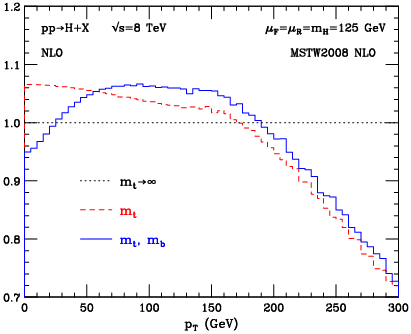
\includegraphics[width=0.5\textwidth]{images/pth_quarkmass.png}
\caption{Distribution of \pth computed at NLO ($\alpha_s^4$) and divided by the calculation obtained in the large-$m_\mathrm{t}$ approximation. The red dashed line corresponds to the calculation including the top quark mass while the blue line refers to the calculation including also the bottom quark effects.}\label{fig:pth_quarkmass}
\end{figure}

Possible extensions of the SM predict a modification of the Higgs boson couplings to gluons and to the top quark. Many of these models actually predict the existence of new states that interact with the SM Higgs boson, but are beyond the direct production reach at the actual LHC energies. The effect of these new states could however show up as a deviation of the Higgs boson couplings with respect to the SM expectation. The modification of the couplings, as shown in Refs.~\cite{Azatov:2013xha,Harlander:2013oja}, can change the kinematics of the Higgs boson production and the effect can be particularly sizeable in the tail of the \pth distribution. 
Other models, such as Composite Higgs~\cite{Marzocca:2012zn}, predict the existence of top-partners, which are heavy resonances with the same quantum numbers as the top quark, that can interact with the Higgs boson in the ggH fermionic loop, changing the \pth shape with respect to what the SM predicts~\cite{Banfi:2013yoa}.
The measurement of the \pth spectrum is thus a useful tool for indirect searches of new particles predicted by theories beyond the SM.
\end{comment}

Measurements of the fiducial cross sections and of several differential
distributions, using the $\sqrt{s}=8$\TeV LHC data, have been reported by ATLAS~\cite{Aad:2014tca,Aad:2014lwa,Aad:2015lha} and CMS~\cite{Khachatryan:2015rxa,Khachatryan:2015yvw} for the ${\mathrm{H} \to \mathrm{ZZ} \to 4\ell}$ ($\ell = \mathrm{e},\mu$) and H $\to \gamma\gamma$ decay channels. In this chapter a measurement of the fiducial cross section times branching fraction ($\sigma \times \mathcal{B}$) and \pt{} spectrum for Higgs boson production in \ensuremath{\mathrm{H}\rightarrow{}\WW\rightarrow \mathrm{e}^{\pm} \mu^{\mp}\nu\nu} ~decays, based on $\sqrt{s} = 8$\TeV LHC data, is reported.

The analysis is performed looking at different flavour leptons in the final state in order to suppress the sizeable contribution of backgrounds containing a same-flavour lepton pair originating from Z boson decay.

Although the \hwwllnn{} channel has lower resolution in the \pth{} measurement
compared to the H $\to \gamma\gamma$ and  H $\to \rm{ZZ}\to 4\ell$ channels
because of neutrinos in the final state, the channel has a significantly
larger $\sigma \times \mathcal{B}$, exceeding those for H $\to \gamma\gamma$ by a factor
of 10 and H $\to \rm{ZZ}\to 4\ell$ by a factor of 85 for a Higgs boson mass of
125\GeV~\cite{Heinemeyer:2013tqa}, and is characterized by good signal
sensitivity. Such sensitivity allowed the observation of a Higgs boson at the level of 4.3 (5.8 expected)
standard deviations for a mass hypothesis of 125.6 GeV using the full LHC data set at 7 and 8\TeV~\cite{Chatrchyan:2013iaa}.

The measurement is performed in a fiducial phase space defined by kinematic requirements on
the leptons that closely match the experimental event selection.

The effect of the limited detector resolution, as well as the
selection efficiency with respect to the fiducial phase space are corrected to
particle level with an unfolding procedure~\cite{Cowan:2002in}, as explained in Sec.~\ref{sec:Unfolding}.


